\section{Linear Texture Mapping}

In this part we tried to overview the ITU logo on the image sequence of ground floor. For this we used the same code from simpleTextureMap function and declare the texturemapGroundFloor method with the implementation for overviewing the logo on each frame of the sequence by using four mouse input points from the first frame.

\begin{figure}[h!]
	\centering
	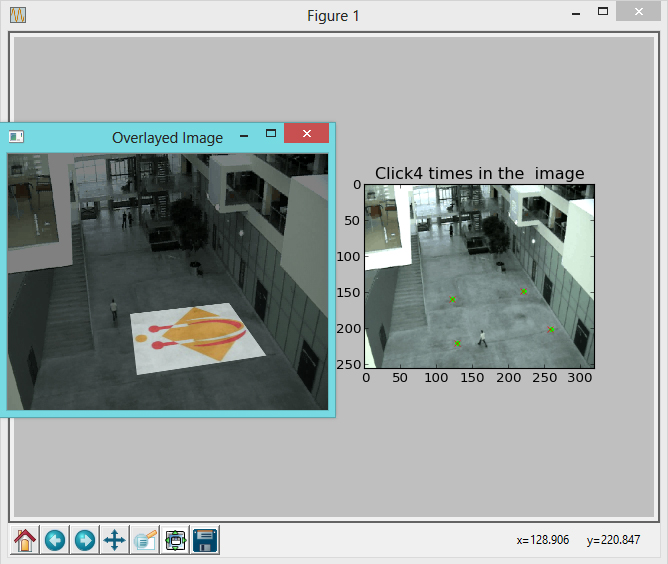
\includegraphics[width=\textwidth]{Handin2/images/linearmapping.jpg}
	\caption{Trace Map}
	\label{fig:trace}
\end{figure}
